\subsection{GitHub Actions}

Afin de garantir le bon fonctionnement du code présent sur la branche \href{https://github.com/Gr4-M3ACNL/hashi/tree/dev}{develop} et, par extension, sur la branche \href{https://github.com/Gr4-M3ACNL/hashi/tree/master}{master}, il est essentiel de s'assurer que chaque nouvelle branche repose sur une base stable. Pour ce faire, nous avons décidé d'automatiser les différentes validations grâce à GitHub Actions, comme illustré dans l'exemple \hyperlink{imgActionCheck}{\emph{ci-dessous}}.

\begin{center}
    \hypertarget{imgActionCheck}{
         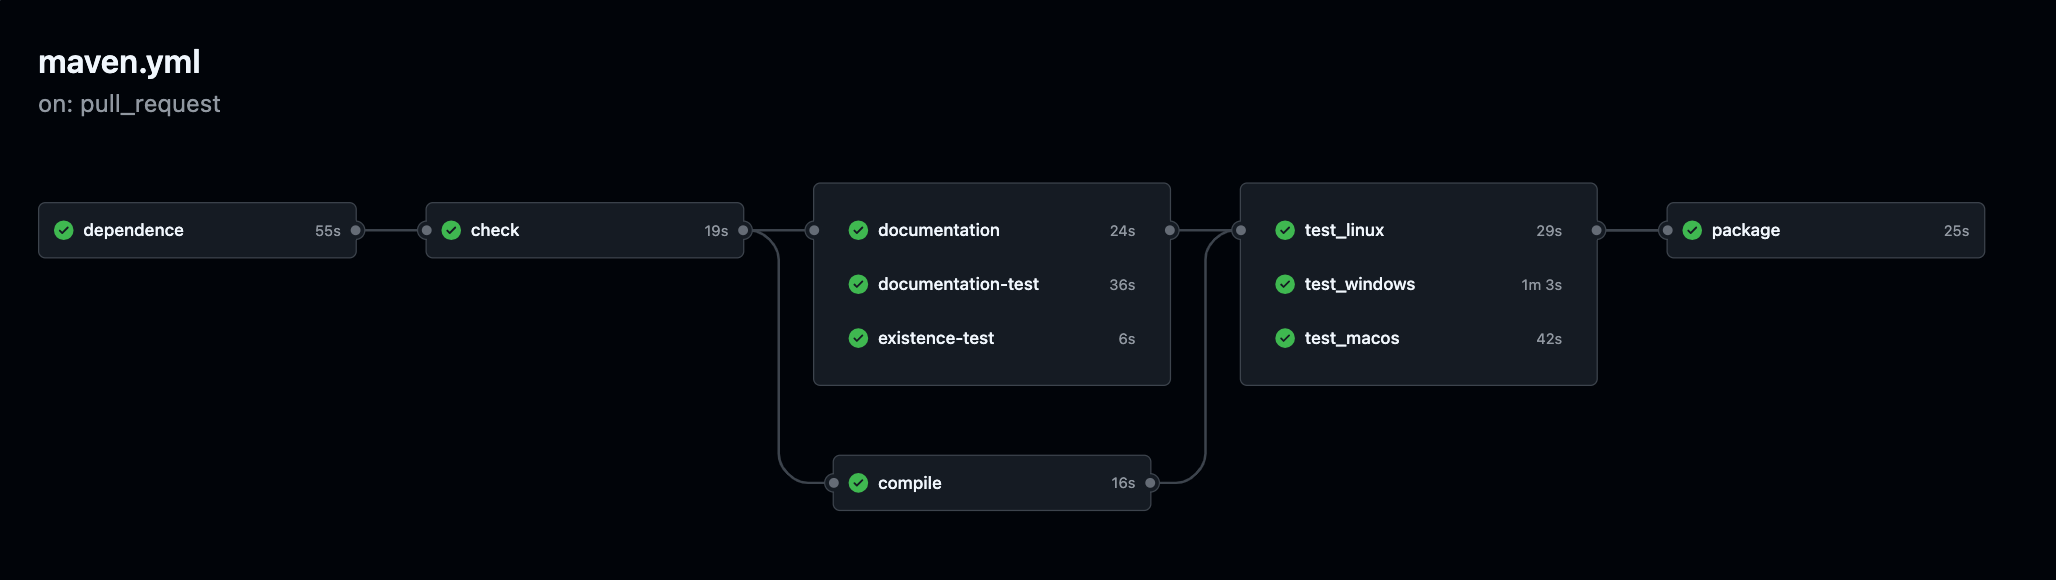
\includegraphics[width=15cm]{../Annexe/git_action_check.png}
    }
\end{center}

Comme on peut l'observer dans l'image \hyperlink{imgActionCheck}{\emph{ci-dessus}}, la validation s'effectue lors d'une \emph{pull request} et se déroule en plusieurs étapes :

\begin{itemize}
    \item \hypertarget{DependenceAction}{\textbf{Dependence}} : Télécharge toutes les dépendances Maven nécessaires aux étapes suivantes.
    \item \hypertarget{CheckAction}{\textbf{Check}} : Vérifie la conformité du code aux règles définies par Checkstyle. Cette étape est indispensable pour toutes les étapes suivantes.
    \item \hypertarget{CompileAction}{\textbf{Compile}} : Dépend de l'étape \hyperlink{CheckAction}{\textbf{Check}} et s'assure que le code peut être compilé sans erreur.
    \item \textbf{Documentation} : Dépend de \hyperlink{CompileAction}{\textbf{Compile}}. Vérifie la possibilité de générer la \emph{Javadoc} pour les classes et bloque la compilation si des classes ou méthodes ne possèdent pas de commentaires correctement formatés.
    \item \textbf{Documentation-Test} : Dépend de \hyperlink{CompileAction}{\textbf{Compile}}. Vérifie la génération de la \emph{Javadoc} pour les classes de test et bloque en cas d'absence de commentaires formatés.
    \item \textbf{Test-Linux} : Dépend de \hyperlink{CompileAction}{\textbf{Compile}}. Exécute l’ensemble des tests sous un environnement \textbf{Linux}. L'échec d’un seul test bloque la validation.
    \item \textbf{Test-Windows} : Dépend de \hyperlink{CompileAction}{\textbf{Compile}}. Exécute l’ensemble des tests sous un environnement \textbf{Windows}. Tout test échoué entraîne un blocage.
    \item \textbf{Test-Macos} : Dépend de \hyperlink{CompileAction}{\textbf{Compile}}. Exécute l’ensemble des tests sous un environnement \textbf{macOS}. Un seul échec empêche la validation.
    \item \textbf{Package} : Dépend de toutes les validations précédentes. Vérifie la capacité du code à générer un \textbf{JAR}, garantissant ainsi que le projet est livrable.
\end{itemize}

Si l'une de ces étapes échoue, la \emph{pull request} est bloquée jusqu'à la correction du problème.

\\
La gestion d'une GitHub Action se fait via un fichier \textbf{YML}, dans lequel les différentes tâches sont configurées sous forme de \emph{jobs}, chacun contenant les étapes nécessaires à son exécution.
\\
Nous avons également utilisé GitHub Actions pour automatiser la génération et la publication de la \emph{Javadoc} lors d'un \emph{push} sur la branche \href{https://github.com/Gr4-M3ACNL/hashi/tree/master}{master}.

\begin{center}
    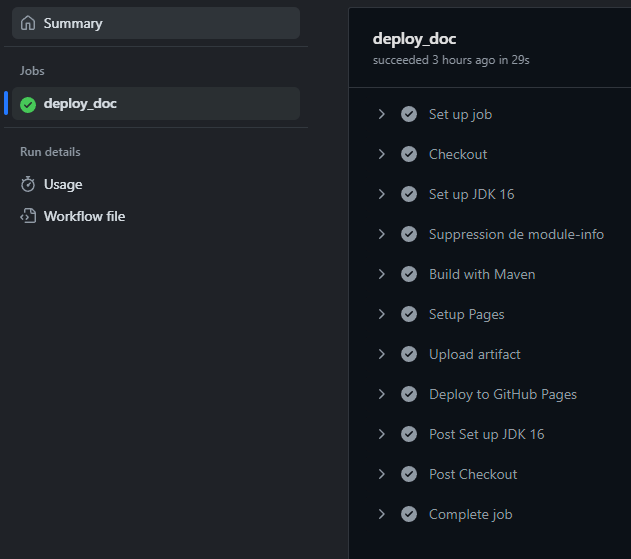
\includegraphics[width=10cm]{../Annexe/git_action_doc.png}
\end{center}
